\section{Advanced Particle Filters}\label{sec:particle_filtering}

Even though the SIR applies under very mild assumptions, it has several caveats. Indeed, while resampling at every step eliminates the weight degeneracy of the SIS, it wastes computational load, and erodes particle diversity. Furthermore, the number of particles required grows quickly with the state dimension, a phenomenon known as the curse of dimensionality \cite{bib:PF-dimension}.

The SIR admits several refinements \cite{bib:beyond-Kalman}, each targeting a specific issue. We first present the generic particle filter, which reduces the SIR's computational cost by only resampling when necessary. We then introduce the regularised and auxiliary particle filters to restore particle diversity and improve on the prior proposal. Finally, we derive the equations of the Rao-Blackwellised particle filter, which reduces the dimension of the explored space under linear-Gaussian substructure assumptions.

\subsection{Generic Particle Filter}

The SIR resamples at every time step, which eliminates weight degeneracy but comes with two drawbacks:
\begin{itemize}
	\item It introduces unnecessary computational cost when weights are already well-distributed, and increases the variance of the estimated state, as mentioned by \Cref{th:loss_independence}.
	\item It also replicates the heaviest particles and discards the lightest, so the set progressively concentrates on a few distinct locations. This loss of diversity, known as particle impoverishment \cite{bib:degeneracy}, is especially severe in low evolution noise or high-dimensional settings, where little diversity is re-introduced at the propagation step. It is illustrated by \Cref{fig:impoverishment}.
\end{itemize}

\begin{figure}[!htb]
	\centering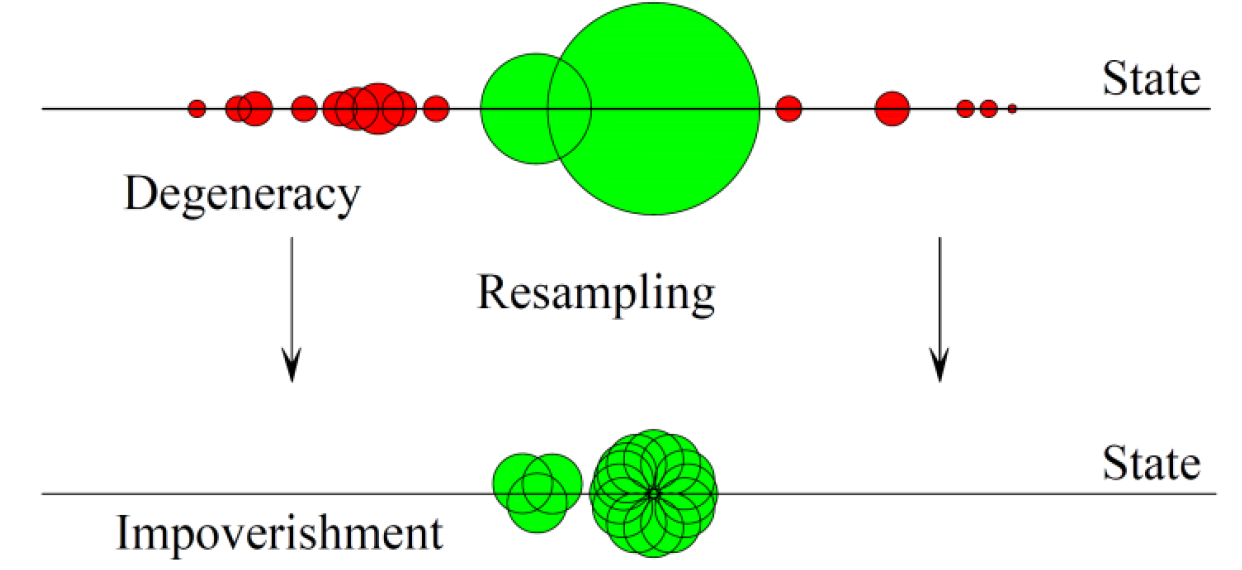
\includegraphics[width=0.6\textwidth]{../../Images/Appauvrissement particulaire.png}
	\caption{Particle impoverishment after resampling. Discarding non-resampled particles progressively shrinks the support of the particle approximation, degrading the filter's ability to explore the state-space.}\label{fig:impoverishment}
\end{figure}

To limit both issues, the generic particle filter (PF) \cite{bib:PF-Sarkka} resamples only when the weight distribution has degraded significantly. This degradation is measured by the effective sample size:
\begin{equation}
	N_{\mathrm{eff}}\triangleq\frac{N}{1+\mathbb{V}_{q(\cdot|\mathbf{z}_{1:k})}\left[\dfrac{p(\mathbf{x}_{0:k}|\mathbf{z}_{1:k})}{q(\mathbf{x}_{0:k}|\mathbf{z}_{1:k})}\right]}
\end{equation}

Its denominator increases with the variance of the importance weights, whose growth over time corresponds to the weight degeneracy characterised by \Cref{th:variance_weights}. When all the weights are uniform, the variance is zero, and thus $N_{\mathrm{eff}}=N$. Conversely, the more unevenly they are distributed, the smaller $N_{\mathrm{eff}}$, with $N_{\mathrm{eff}}\to1$ when the mass concentrates on a single particle.

Since the true importance weights are unknown, $N_{\mathrm{eff}}$ is estimated by replacing $\mathbb{V}_{q(\cdot|\mathbf{z}_{1:k})}[\cdot]$ with the empirical spread of the normalised weights \cite{bib:SMC-dynamic}, which gives:
\begin{equation}
	\hat{N}_{\mathrm{eff}}\triangleq\frac{1}{\displaystyle\sum_{i=1}^N\left(w_k^{(i)}\right)^2}\leq N
\end{equation}

Like $N_{\mathrm{eff}}$, this quantity ranges from $N$ for uniform weights, down to $1$ in the fully degenerate case. The PF then performs the resampling step only when this estimate falls below a threshold:
\begin{equation}
	\hat{N}_{\mathrm{eff}}<N_{\mathrm{th}}
\end{equation}
where $N_{\mathrm{th}}$ is a predetermined value, typically chosen proportional to $N$.

Unlike the SIR, which traditionally uses the transition density as its proposal distribution, the generic PF is not typically restricted to any particular choice of proposal distribution. It is presented by \Cref{alg:PF}.

\begin{algorithm}[!htb]
	\begin{algorithmic}
	\State{$\forall i\in[\![1,N]\!],\:x_k^{(i)}\sim q\left(\cdot|x_{k-1}^{(i)},z_k\right)$}\Comment{Particle propagation}
	\State{$\forall i\in[\![1,N]\!],\:\tilde{w}_k^{(i)}=w_{k-1}^{(i)}\:\dfrac{\tilde{p}\left(z_k|x_k^{(i)}\right)\:\tilde{p}\left(x_k^{(i)}|x_{k-1}^{(i)}\right)}{\tilde{q}\left(x_k^{(i)}|\mathbf{x}_{0:k-1}^{(i)},\mathbf{z}_{1:k}\right)}$}\Comment{Weight update}
	\State{$\displaystyle\forall i\in[\![1,N]\!],\:w_k^{(i)}=\left.\tilde{w}_k^{(i)}\middle/\sum_{j=1}^N\tilde{w}_k^{(j)}\right.$}\Comment{Normalisation}
	\State{$\displaystyle\hat{N}_{\mathrm{eff}}=\left.1\middle/\sum_{i=1}^N\left(w_k^{(i)}\right)^2\right.$}\Comment{Resampling criterion}
	\If{$\hat{N}_{\mathrm{eff}}<N_{\mathrm{th}}$}
	\State{$\left\{x_k^{(j)},w_k^{(j)},-\right\}_{j=1}^N\gets\operatorname{Resampling}\left(\left\{x_k^{(i)},w_k^{(i)}\right\}_{i=1}^N\right)$}\Comment{Resampling}
	\EndIf
	\end{algorithmic}\caption{Generic Particle Filter}\label{alg:PF}
\end{algorithm}

\subsection{Regularised Particle Filter}

Since each resampling step still collapses diversity, the PF only mitigates impoverishment, but does not prevent it. Indeed, the self-normalised measure of \Cref{th:self_normalised_measure} approximates the PDF by a mixture of Diracs:
\begin{equation}
	p(x_k|\mathbf{z}_{1:k})\:dx_k\approx\sum_{i=1}^Nw_k^{(i)}\:\delta_{x_k^{(i)}}\label{eq:RPF_dirac}
\end{equation}

Since this measure is singular, resampling from it can only reproduce the existing particles. The regularised particle filter (RPF) \cite{bib:RPF} addresses this issue through kernel density estimation \cite{bib:Rosenblatt,bib:Parzen,bib:Silverman}, by replacing each Dirac with a smooth kernel to obtain the absolutely continuous measure:
\begin{equation}
	p(x_k|\mathbf{z}_{1:k})\:dx_k\approx\sum_{i=1}^Nw_k^{(i)}\:K_h\left(x_k-x_k^{(i)}\right)dx_k\label{eq:RPF_kernel}
\end{equation}

New particles are then drawn from this continuous density rather than from the discrete set, which restores diversity, as illustrated by \Cref{fig:regularisation} and formalised by \Cref{th:regularisation_kernel,th:KDE}. Being absolutely continuous, this approximation also supplies the density that \eqref{eq:RPF_dirac} lacks, and thus makes the MAP estimator of \cref{sec:state_estimation} well-defined at the cost of a numerical maximisation.

\begin{figure}[!htb]
	\centering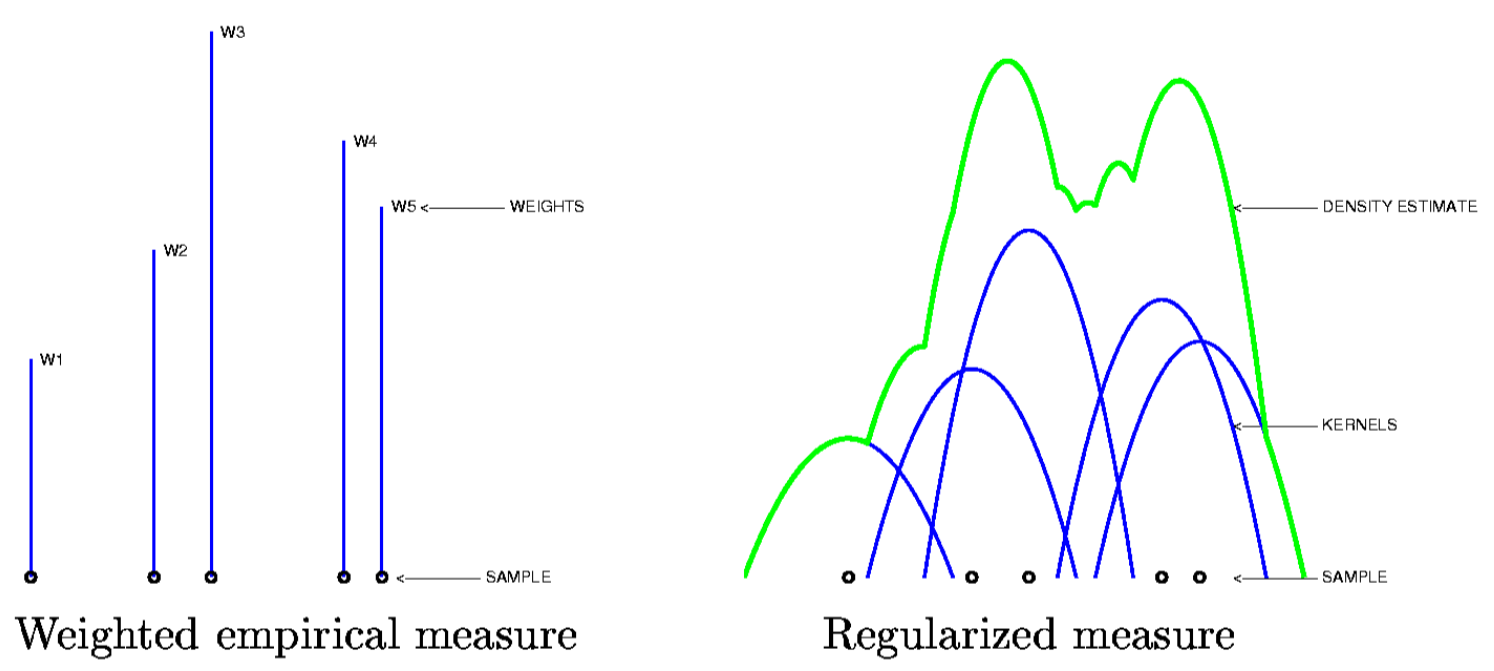
\includegraphics[width=0.8\textwidth]{../../Images/Régularisation par noyau.png}
	\caption{An example Monte Carlo approximation of the PDF \eqref{eq:RPF_dirac} on the left and its kernel regularisation \eqref{eq:RPF_kernel} on the right, for a given particle set. The latter approximation bridges the gaps between particles and spans a larger region of the state space.}\label{fig:regularisation}
\end{figure}

\begin{definition}[Regularisation kernels]\label{th:regularisation_kernel}
	Let $K:\mathbb{R}^{d_x}\to\mathbb{R}$. $K$ is a regularisation kernel if:
	\begin{equation}
		\left\{\begin{array}{ll}
		\forall x\in\mathbb{R}^{d_x},\:K(x)\geq0&\text{positive}\\
		\forall x\in\mathbb{R}^{d_x},\:K(-x)=K(x)&\text{symmetric}\\
		\displaystyle\int{K(x)\:dx}=1&\text{normalised}\\
		\displaystyle\int{\|x\|^2K(x)\:dx}<\infty&\text{of finite variance}
		\end{array}\right.
	\end{equation}

	Furthermore, for $K$ a regularisation kernel and $h>0$, we define the rescaled kernel $K_h$ of bandwidth $h$ as:
	\begin{equation}
		K_h:\left\{\begin{aligned}
		\mathbb{R}^{d_x}&\to\mathbb{R}\\
		x&\mapsto\frac{1}{h^{d_x}}K\left(\frac{x}{h}\right)
		\end{aligned}\right.
	\end{equation}
\end{definition}

\begin{definition}[Regularised estimator]\label{th:KDE}
	Let $*$ denote the convolution operator. The regularised measure $S_{K_h}^N$ of some empirical measure $S^N$ with respect to a regularisation kernel $K_h$ is:
	\begin{equation}
		S_{K_h}^N(\mu)\triangleq K_h*S^N(\mu)
	\end{equation}

	In particular, the regularised self-normalised estimator verifies:
	\begin{equation}
		\tilde{S}_{K_h}^N(\mu,\nu)=\sum_{i=1}^Nw^{(i)}\:\left(K_h*\delta_{X^{(i)}}\right)
	\end{equation}
	and the corresponding estimator is:
	\begin{equation}
		\left\langle\tilde{S}_{K_h}^N(\mu,\nu),\varphi\right\rangle=\sum_{i=1}^Nw^{(i)}\:\left(K_h*\varphi\right)\left(X^{(i)}\right)
	\end{equation}
	by symmetry of $K_h$.
\end{definition}

The choice of bandwidth $h$ is critical to the performance of the RPF. If $h$ is too small, $K_h$ concentrates around the Dirac measure, and the regularisation has no practical effect on particle diversity. Conversely, the kernel density estimate over-smooths the posterior when $h$ is too large, artificially spreading particles across regions of low probability, and degrading filter accuracy. In this section, we present two classical choices for $K_h$:
\begin{itemize}
	\item\textbf{Epanechnikov kernel \cite{bib:Epanechnikov}.} This kernel minimises the mean integrated squared error (MISE) among all regularisation kernels, and the associated bandwidth is optimal when the density is Gaussian with identity covariance. It is defined by:
	\begin{equation}
		\left\{\begin{aligned}
		K_{\mathrm{Epa}}&:x\mapsto\frac{d_x+2}{2c_{d_x}}\left(1-\|x\|^2\right)\mathbbm{1}_{\|x\|\leq1}(x)\\
		h_{\mathrm{Epa}}&=\left(\frac{8(d_x+4)\left(2\sqrt{\pi}\right)^{d_x}}{c_{d_x}}\right)^{\frac{1}{d_x+4}}N^{-\frac{1}{d_x+4}}
		\end{aligned}\right.
	\end{equation}
	where:
	\begin{equation}
		c_{d_x}\triangleq\frac{\pi^{d_x/2}}{\Gamma(d_x/2+1)}
	\end{equation}
	is the volume of the $\mathbb{R}^{d_x}$ unit ball, and $\Gamma$ is the Gamma function.
	\item\textbf{Gaussian kernel.} While suboptimal with respect to the Epanechnikov kernel, it is simpler to compute \cite{bib:random-variate}. Its expression is given by:
	\begin{equation}
		\left\{\begin{aligned}
		K_{\mathrm{Gauss}}&:x\mapsto(2\pi)^{-d_x/2}\exp\left(-\frac{\|x\|^2}{2}\right)\\
		h_{\mathrm{Gauss}}&=\left(\frac{4}{d_x+2}\right)^{\frac{1}{d_x+4}}N^{-\frac{1}{d_x+4}}
		\end{aligned}\right.
	\end{equation}
\end{itemize}

It must be noted that the assumptions for the Epanechnikov, and consequently the Gaussian, regularisation are not usually met in practice, since MC methods are precisely used when the PDF is not Gaussian.

However, the two conditions do not play the same role. The Gaussian hypothesis is only used to compute the optimal bandwidth, whose expression would otherwise depend on an unknown PDF. It is thus a calibration convention rather than a modelling assumption. In particular, it tends to overestimate $h$ when the PDF is multimodal.

On the other hand, the unit covariance is a scaling requirement, and can be enforced exactly by a whitening step before the regularisation. This amounts to replacing every particle by $A_k^{-1}\:x_k^{(i)}$, where $A_k$ is the Cholesky factor \cite{bib:matrix-computations} of $\hat{P}_k$:
\begin{equation}
	\hat{P}_k=A_k\:A_k^\top
\end{equation}
which ensures that the covariance matrix of the new particle set is the identity. While seemingly computationally heavy, this reduces to using the following regularisation kernel on the standard particle set:
\begin{equation}
	\tilde{K}_h:x\mapsto\frac{\det(A_k)^{-1}}{h^{d_x}}K\left(\frac{1}{h}A_k^{-1}x\right)
\end{equation}

Moreover, the bandwidth $h$ is multiplied by a modulation factor $\alpha_{\mathrm{reg}}\in[0,1]$ to avoid over-smoothing in cases where the PDF is multimodal. The pseudo-code for the RPF is given by \Cref{alg:RPF}.

\begin{algorithm}[!htb]
	\begin{algorithmic}
	\State{$\forall i\in[\![1,N]\!],\:x_k^{(i)}\sim q\left(\cdot|x_{k-1}^{(i)},z_k\right)$}\Comment{Particle propagation}
	\State{$\forall i\in[\![1,N]\!],\:\tilde{w}_k^{(i)}=w_{k-1}^{(i)}\:\dfrac{\tilde{p}\left(z_k|x_k^{(i)}\right)\:\tilde{p}\left(x_k^{(i)}|x_{k-1}^{(i)}\right)}{\tilde{q}\left(x_k^{(i)}|\mathbf{x}_{0:k-1}^{(i)},\mathbf{z}_{1:k}\right)}$}\Comment{Weight update}
	\State{$\displaystyle\forall i\in[\![1,N]\!],\:w_k^{(i)}=\left.\tilde{w}_k^{(i)}\middle/\sum_{j=1}^N\tilde{w}_k^{(j)}\right.$}\Comment{Normalisation}
	\State{$\displaystyle\hat{N}_{\mathrm{eff}}=\left.1\middle/\sum_{i=1}^N\left(w_k^{(i)}\right)^2\right.$}\Comment{Resampling criterion}
	\If{$\hat{N}_{\mathrm{eff}}<N_{\mathrm{th}}$}
	\State{$\displaystyle\hat{x}_k=\sum_{i=1}^Nw_k^{(i)}x_k^{(i)}$}\Comment{Whitening}
	\State{$\displaystyle\hat{P}_k=\sum_{i=1}^Nw_k^{(i)}\left(x_k^{(i)}-\hat{x}_k\right)\left(x_k^{(i)}-\hat{x}_k\right)^\top$}
	\State{$A_k\text{ s.t. }\hat{P}_k=A_k\:A_k^\top$}
	\State{$\left\{x_k^{(j)},w_k^{(j)},-\right\}_{j=1}^N\gets\operatorname{Resampling}\left(\left\{x_k^{(i)},w_k^{(i)}\right\}_{i=1}^N\right)$}\Comment{Resampling}
	\State{$\forall j\in[\![1,N]\!],\:\varepsilon^{(j)}\sim K$}\Comment{Regularisation}
	\State{$\forall j\in[\![1,N]\!],\:x_k^{(j)}\gets x_k^{(j)}+\alpha_{\mathrm{reg}}hA_k\:\varepsilon^{(j)}$}
	\EndIf
	\end{algorithmic}\caption{Regularised Particle Filter}\label{alg:RPF}
\end{algorithm}

\subsection{Auxiliary Particle Filter}

The auxiliary particle filter (APF) \cite{bib:APF,bib:APF-optimality} addresses the degeneracy problem at its root by exploiting a different weakness of the SIR. Since particles are propagated before the new observation $z_k$ is taken into account, particles that will ultimately receive low likelihood waste computational effort. The APF thus introduces a look-ahead step by using a prediction of their future likelihood to resample promising parent particles before propagation.

Formally, the APF targets the joint distribution $p(x_k,i|\mathbf{z}_{1:k})$, where $i\in[\![1,N]\!]$ indexes the parent particle at time $k-1$. Using Bayes' theorem and the chain rule gives:
\begin{equation}
	p(x_k,i|\mathbf{z}_{1:k})\propto p(z_k|x_k,i,\mathbf{z}_{1:k-1})\:p(x_k|i,\mathbf{z}_{1:k-1})\:p(i|\mathbf{z}_{1:k-1})\label{eq:joint_distribution_APF}
\end{equation}

Each term of this decomposition can be simplified as follows:
\begin{itemize}
	\item\Cref{th:observation_independence} states that the current observation depends only on the current state:
	\begin{equation}
		p(z_k|x_k,i,\mathbf{z}_{1:k-1})=p(z_k|x_k)
	\end{equation}
	\item Since the parent index uniquely determines the ancestor trajectory, conditioning on $i$ is equivalent to conditioning on $x_{0:k-1}^{(i)}$. Moreover, \Cref{th:Markov} establishes that $(x_k)_{k\geq0}$ is a Markov chain, and thus:
	\begin{equation}
		p(x_k|i,\mathbf{z}_{1:k-1})=p\left(x_k|\mathbf{x}_{0:k-1}^{(i)},\mathbf{z}_{1:k-1}\right)=p\left(x_k|x_{k-1}^{(i)}\right)
	\end{equation}
	\item Finally, assuming that the particle approximation is exact gives:
	\begin{equation}
		p(i|\mathbf{z}_{1:k-1})\propto w_{k-1}^{(i)}
	\end{equation}
\end{itemize}

Combining these equations reduces \eqref{eq:joint_distribution_APF} to:
\begin{equation}
	p(x_k,i|\mathbf{z}_{1:k})\propto p\left(z_k|x_k\right)\:p\left(x_k|x_{k-1}^{(i)}\right)\:w_{k-1}^{(i)}
\end{equation}

However, $p(z_k|x_k)$ cannot be evaluated before $x_k$ is drawn. It is thus approximated by $p\left(z_k|\mu_k^{(i)}\right)$, where:
\begin{equation}
	\mu_k^{(i)}\sim p\left(\cdot|x_{k-1}^{(i)}\right)
\end{equation}
is an auxiliary particle drawn from the transition density, and used to assess the consistency of the future particle $x_k^{(i)}$ with the new observation $z_k$. Alternatively, $\mu_k^{(i)}$ can be chosen as the mean of this density, a deterministic choice which avoids an additional draw.

In any case, the importance density is therefore:
\begin{equation}
	q(x_k,i|\mathbf{z}_{1:k})\propto p\left(z_k|\mu_k^{(i)}\right)\:p\left(x_k|x_{k-1}^{(i)}\right)\:w_{k-1}^{(i)}
\end{equation}

Since they are drawn from the prior distribution, \eqref{eq:weight_update_prior} ensures that the auxiliary weights $\lambda_k^{(i)}$ follow:
\begin{equation}
	\lambda_k^{(i)}\propto w_{k-1}^{(i)}\:\tilde{p}\left(z_k|\mu_k^{(i)}\right)
\end{equation}

In the hope that the evolution noise is sufficiently weak for the auxiliary particles to correctly represent the future particle set, the parent indices $\left\{i^{(j)}\right\}_{j=1}^N$ are resampled according to the auxiliary weights.

The new particle set is then propagated through a standard SIS algorithm using the transition density:
\begin{equation}
	x_k^{(j)}\sim p\left(\cdot|x_{k-1}^{\left(i^{(j)}\right)}\right)
\end{equation}
with their weights updating as:
\begin{equation}
	\begin{aligned}
	w_k^{(j)}&\propto\frac{\tilde{p}\left(x_k,i^{(j)}|\mathbf{z}_{1:k}\right)}{\tilde{q}\left(x_k,i^{(j)}|\mathbf{z}_{1:k}\right)}\\
	&\propto\frac{\tilde{p}\left(z_k|x_k^{(j)}\right)\:\tilde{p}\left(x_k^{(j)}|x_{k-1}^{\left(i^{(j)}\right)}\right)\:w_{k-1}^{\left(i^{(j)}\right)}}{\tilde{p}\left(z_k|\mu_k^{\left(i^{(j)}\right)}\right)\:\tilde{p}\left(x_k^{(j)}|x_{k-1}^{\left(i^{(j)}\right)}\right)\:w_{k-1}^{\left(i^{(j)}\right)}}\\
	&\propto\frac{\tilde{p}\left(z_k|x_k^{(j)}\right)}{\tilde{p}\left(z_k|\mu_k^{\left(i^{(j)}\right)}\right)}
	\end{aligned}
\end{equation}

The full APF algorithm is given in \cref{alg:APF}.

\begin{algorithm}[!htb]
	\begin{algorithmic}
	\State{$\forall i\in[\![1,N]\!],\:\mu_k^{(i)}\sim p\left(\cdot|x_{k-1}^{(i)}\right)$}\Comment{Auxiliary propagation}
	\State{$\forall i\in[\![1,N]\!],\:\tilde{\lambda}_k^{(i)}\propto w_{k-1}^{(i)}\:\tilde{p}\left(z_k|\mu_k^{(i)}\right)$}\Comment{Auxiliary update}
	\State{$\displaystyle\forall i\in[\![1,N]\!],\:\lambda_k^{(i)}=\left.\tilde{\lambda}_k^{(i)}\middle/\sum_{j=1}^N\tilde{\lambda}_k^{(j)}\right.$}\Comment{Normalisation}
	\State{$\left\{-,-,i^{(j)}\right\}_{j=1}^N=\operatorname{Resampling}\left(\left\{\mu_k^{(i)},\lambda_k^{(i)}\right\}_{i=1}^N\right)$}\Comment{Resampling}
	\State{$\forall j\in[\![1,N]\!],\:x_k^{(j)}\sim p\left(\cdot|x_{k-1}^{\left(i^{(j)}\right)}\right)$}\Comment{Particle propagation}
	\State{$\forall j\in[\![1,N]\!],\:\tilde{w}_k^{(j)}\propto\dfrac{\tilde{p}\left(z_k|x_k^{(j)}\right)}{\tilde{p}\left(z_k|\mu_k^{\left(i^{(j)}\right)}\right)}$}\Comment{Weight update}
	\State{$\displaystyle\forall j\in[\![1,N]\!],\:w_k^{(j)}=\left.\tilde{w}_k^{(j)}\middle/\sum_{i=1}^N\tilde{w}_k^{(i)}\right.$}\Comment{Normalisation}
	\end{algorithmic}\caption{Auxiliary Particle Filter}\label{alg:APF}
\end{algorithm}

\begin{remark}[Comparison between the RPF and the APF]
	Both the RPF and the APF aim to alleviate the degeneracy and impoverishment problems of the standard PF, but they target different sources:
	\begin{itemize}
		\item The RPF restores diversity through kernel density estimation, addressing the severe impoverishment caused by near-deterministic dynamics. It is therefore suited to low evolution noise scenarios.
		\item The APF instead pre-selects promising parents from the incoming observation. It is preferred when the observation noise is small, since a peaked likelihood triggers an important single-step weight degeneracy.
	\end{itemize}

	These preferences are rules of thumb rather than theoretical results, and the APF's pre-selection also degrades under strong evolution noise. Acting at different stages, both filters are ultimately complementary rather than exclusive.
\end{remark}

\subsection{Rao-Blackwellised Particle Filter}

The marginalised particle filter \cite{bib:MPF}, also known as the Rao-Blackwellised particle filter (RBPF) \cite{bib:Rao-Blackwellisation,bib:RBPF}, reduces the dimension of the state-space explored by the particle filter by exploiting a partial linear-Gaussian structure in the state-space model. Suppose that the state can be decomposed as:
\begin{equation}
	x_k=\left[x_k^n,x_k^l\right]
\end{equation}
such that \eqref{eq:navigation_problem} is linear and Gaussian in $x_k^l$ conditionally on $x_k^n$. The navigation system can be rewritten as:
\begin{equation}
	(S):\left\{\begin{aligned}
	x_k^n&=F_k^n\left(x_{k-1}^n\right)\:x_{k-1}^l+f_k^n\left(x_{k-1}^n\right)+w_k^n\\
	x_k^l&=F_k^l\left(x_{k-1}^n\right)\:x_{k-1}^l+f_k^l\left(x_{k-1}^n\right)+w_k^l\\
	z_k&=H_k\left(x_k^n\right)\:x_k^l+h_k\left(x_k^n\right)+n_k
	\end{aligned}\right.\label{eq:RBPF_model}
\end{equation}
with:
\begin{equation}
	w_k=\begin{bmatrix}w_k^n\\w_k^l\end{bmatrix}
	\sim\mathcal{N}\left(0,\begin{bmatrix}
	Q_k^n&(Q_k^{nl})^\top\\Q_k^{nl}&Q_k^l
	\end{bmatrix}\right),\quad n_k\sim\mathcal{N}(0,R_k)
\end{equation}
$x_0^n$ of known distribution, and $x_0^l$ Gaussian.

The idea behind the RBPF is to factorise the PDF as:
\begin{equation}
	p\left(\mathbf{x}_{0:k}^l,\mathbf{x}_{0:k}^n|\mathbf{z}_{1:k}\right)=p\left(\mathbf{x}_{0:k}^l|\mathbf{x}_{0:k}^n,\mathbf{z}_{1:k}\right)\:p\left(\mathbf{x}_{0:k}^n|\mathbf{z}_{1:k}\right)
\end{equation}
where $p(\mathbf{x}_{0:k}^n|\mathbf{z}_{1:k})$ is estimated via particle filtering techniques, and $p(\mathbf{x}_{0:k}^l|\mathbf{x}_{0:k}^n,\mathbf{z}_{1:k})$ is analytically solved by a Kalman filter. Here, $\mathbf{x}_{0:k}^l$ and $\mathbf{x}_{0:k}^n$ are defined similarly to $\mathbf{x}_{0:k}$.

When $Q_k^{nl}\neq 0$, the noises $w_k^l$ and $w_k^n$ are correlated, and the Kalman filter cannot be applied directly. \Cref{th:RBPF_decorrelation} decouples them by removing the component of $w_k^l$ correlated with $w_k^n$.

\begin{proposition}[Noise decorrelation]\label{th:RBPF_decorrelation}
	The decorrelated noise:
	\begin{equation}
		\overline{w}_k^l\triangleq w_k^l-Q_k^{nl}\:(Q_k^n)^{-1}\:w_k^n
	\end{equation}
	is centred, uncorrelated with $w_k^n$, and has covariance:
	\begin{equation}
		\overline{Q}_k^l\triangleq\mathbb{V}\left[\overline{w}_k^l\right]=Q_k^l-Q_k^{nl}\:(Q_k^n)^{-1}\:(Q_k^{nl})^\top
	\end{equation}
\end{proposition}

\begin{proof}
	As a linear combination of the centred noises $w_k^l$ and $w_k^n$, $\overline{w}_k^l$ is centred. Its covariance develops as:
	\begin{equation}
		\begin{aligned}
		\overline{Q}_k^l&=\mathbb{E}\left[\overline{w}_k^l\:{\overline{w}_k^l}^\top\right]\\
		&=\mathbb{E}\left[(w_k^l-Q_k^{nl}\:(Q_k^n)^{-1}\:w_k^n)\:(w_k^l-Q_k^{nl}\:(Q_k^n)^{-1}\:w_k^n)^\top\right]\\
		&=\mathbb{E}\left[w_k^l\:(w_k^l)^\top\right]-\mathbb{E}\left[w_k^l\:(Q_k^{nl}\:(Q_k^n)^{-1}\:w_k^n)^\top\right]-\mathbb{E}\left[(Q_k^{nl}\:(Q_k^n)^{-1}\:w_k^n)\:(w_k^l)^\top\right]\\
		&\qquad+\mathbb{E}\left[(Q_k^{nl}\:(Q_k^n)^{-1}\:w_k^n)\:(Q_k^{nl}\:(Q_k^n)^{-1}\:w_k^n)^\top\right]\\
		&=\mathbb{E}\left[w_k^l\:(w_k^l)^\top\right]-\mathbb{E}\left[w_k^l\:(w_k^n)^\top\right](Q_k^n)^{-\top}\:(Q_k^{nl})^\top-Q_k^{nl}\:(Q_k^n)^{-1}\:\mathbb{E}\left[w_k^n\:(w_k^l)^\top\right]\\
		&\qquad+Q_k^{nl}\:(Q_k^n)^{-1}\:\mathbb{E}\left[w_k^n\:(w_k^n)^\top\right]\:(Q_k^n)^{-\top}\:(Q_k^{nl})^\top\\
		&=Q_k^l-Q_k^{nl}\:(Q_k^n)^{-\top}\:(Q_k^{nl})^\top-Q_k^{nl}\:(Q_k^n)^{-1}\:(Q_k^{nl})^\top+Q_k^{nl}\:(Q_k^n)^{-1}\:Q_k^n\:(Q_k^n)^{-\top}\:(Q_k^{nl})^\top\\
		&=Q_k^l-Q_k^{nl}\:(Q_k^n)^{-1}\:(Q_k^{nl})^\top-Q_k^{nl}\:(Q_k^n)^{-1}\:(Q_k^{nl})^\top+Q_k^{nl}\:(Q_k^n)^{-1}\:(Q_k^{nl})^\top\\
		&=Q_k^l-Q_k^{nl}\:(Q_k^n)^{-1}\:(Q_k^{nl})^\top
		\end{aligned}
	\end{equation}

	Finally, computing:
	\begin{equation}
		\begin{aligned}
		\mathbb{E}\left[\overline{w}_k^l\:(w_k^n)^\top\right]&=\mathbb{E}\left[(w_k^l-Q_k^{nl}\:(Q_k^n)^{-1}\:w_k^n)\:(w_k^n)^\top\right]\\
		&=\mathbb{E}\left[w_k^l\:(w_k^n)^\top\right]-Q_k^{nl}\:(Q_k^n)^{-1}\:\mathbb{E}\left[w_k^n\:(w_k^n)^\top\right]\\
		&=Q_k^{nl}-Q_k^{nl}\:(Q_k^n)^{-1}\:Q_k^n\\
		&=0
		\end{aligned}
	\end{equation}
	shows that $\overline{w}_k^l$ and $w_k^n$ are uncorrelated.
\end{proof}

Let:\begin{align}
	\overline{F}_k^l(x_{k-1}^n)&\triangleq F_k^l(x_{k-1}^n)-Q_k^{nl}\:(Q_k^n)^{-1}F_k^n(x_{k-1}^n)\\
	\overline{f}_k^l(x_{k-1}^n)&\triangleq f_k^l(x_{k-1}^n)-Q_k^{nl}\:(Q_k^n)^{-1}f_k^n(x_{k-1}^n)
\end{align}

The system \eqref{eq:RBPF_model} can be rewritten as:
\begin{equation}
	\left(\overline{S}\right):\left\{\begin{aligned}
	x_k^n&=F_k^n\left(x_{k-1}^n\right)\:x_{k-1}^l+f_k^n\left(x_{k-1}^n\right)+w_k^n\\
	x_k^l&=\overline{F}_k^l\left(x_{k-1}^n\right)\:x_{k-1}^l+\overline{f}_k^l\left(x_{k-1}^n\right)+Q_k^{nl}\:(Q_k^n)^{-1}\:x_k^n+\overline{w}_k^l\\
	z_k&=H_k\left(x_k^n\right)\:x_k^l+h_k\left(x_k^n\right)+n_k
	\end{aligned}\right.
\end{equation}
which can in turn be decomposed as:
\begin{equation}
	\begin{aligned}
	(S_1)&:\left\{\begin{aligned}
	x_{k-1}^l&=x_{k-1}^l\\
	x_k^n&=F_k^n\left(x_{k-1}^n\right)\:x_{k-1}^l+f_k^n\left(x_{k-1}^n\right)+w_k^n\\
	\end{aligned}\right.\\
	(S_2)&:\left\{\begin{aligned}
	x_k^l&=\overline{F}_k^l\left(x_{k-1}^n\right)\:x_{k-1}^l+\overline{f}_k^l\left(x_{k-1}^n\right)+Q_k^{nl}\:(Q_k^n)^{-1}\:x_k^n+\overline{w}_k^l\\
	z_k&=H_k\left(x_k^n\right)\:x_k^l+h_k\left(x_k^n\right)+n_k
	\end{aligned}\right.
	\end{aligned}
\end{equation}

Note the similarities between each of the systems $(S_1)$ and $(S_2)$, and the navigation equations under Kalman hypotheses \eqref{eq:navigation_Kalman}. Indeed, $(S_1)$ can be treated as if the propagation of the non-linear state $x_k^n$ were an observation of $x_{k-1}^l$. Its absence of dynamics leads to only performing the (pre-)correction step of the Kalman filter. On the other hand, $(S_2)$ can be handled by the usual Kalman prediction/correction.

In full generality, a standard RBPF is computed in five steps:
\begin{itemize}
	\item\textbf{Particle propagation.} The non-linear state is propagated according to the proposal density:
	\begin{equation}
		{x_k^n}^{(i)}\sim q\left(\cdot|{x_{k-1}^n}^{(i)},z_k\right)\label{eq:RBPF_propagation}
	\end{equation}
	\item\textbf{Kalman pre-correction.} The previous linear state is corrected according to the Kalman equations applied to $(S_1)$:
	\begin{align}
		\tilde{F}_k^{n(i)}&=F_k^n\left(x_{k-1}^{n(i)}\right)\label{eq:RBPF_precorrection_debut}\\
		y_k^{n(i)}&=x_k^{n(i)}-\left(\tilde{F}_k^{n(i)}\:\hat{x}_{k-1|k-1}^{l(i)}+f_k^n\left(x_{k-1}^{n(i)}\right)\right)\\
		S_k^{n(i)}&=\tilde{F}_k^{n(i)}\:P_{k-1|k-1}^{l(i)}\left(\tilde{F}_k^{n(i)}\right)^\top+Q_k^n\\
		K_k^{n(i)}&=P_{k-1|k-1}^{l(i)}\left(\tilde{F}_k^{n(i)}\right)^\top\left(S_k^{n(i)}\right)^{-1}\\
		\hat{x}_{k-1|k-1}^{l(i)}&\gets\hat{x}_{k-1|k-1}^{l(i)}+K_k^{n(i)}\:y_k^{n(i)}\\
		P_{k-1|k-1}^{l(i)}&\gets\left(I-K_k^{n(i)}\:\tilde{F}_k^{n(i)}\right)P_{k-1|k-1}^{l(i)}\label{eq:RBPF_precorrection_fin}
	\end{align}
	\item\textbf{Kalman prediction.} The current linear state is then predicted via the dynamics of $(S_2)$:
	\begin{align}
		\tilde{F}_k^{l(i)}&=\overline{F}_k^l\left(x_{k-1}^{n(i)}\right)\label{eq:RBPF_prediction_debut}\\
		\hat{x}_{k|k-1}^{l(i)}&=\tilde{F}_k^{l(i)}\:\hat{x}_{k-1|k-1}^{l(i)}+\overline{f}_k^l\left(x_{k-1}^{n(i)}\right)+Q_k^{nl}\:(Q_k^n)^{-1}\:x_k^{n(i)}\\
		P_{k|k-1}^{l(i)}&=\tilde{F}_k^{l(i)}\:P_{k-1|k-1}^{l(i)}\:\left(\tilde{F}_k^{l(i)}\right)^\top+\overline{Q}_k^l\\
		\tilde{H}_k^{(i)}&=H_k\left(x_k^{n(i)}\right)\\
		y_k^{l(i)}&=z_k-\left(\tilde{H}_k^{(i)}\:\hat{x}_{k|k-1}^{l(i)}+h_k\left(x_k^{n(i)}\right)\right)\\
		S_k^{l(i)}&=\tilde{H}_k^{(i)}\:P_{k|k-1}^{l(i)}\left(\tilde{H}_k^{(i)}\right)^\top+R_k\label{eq:RBPF_prediction_fin}
	\end{align}
	\item\textbf{Weight update.} The weights corresponding to each particle are updated with respect to the new observation:
	\begin{align}
		\tilde{w}_k^{n(i)}&=w_{k-1}^{n(i)}\:\dfrac{\tilde{p}\left(z_k|x_k^{n(i)}\right)\:\tilde{p}\left(x_k^{n(i)}|x_{k-1}^{n(i)}\right)}{\tilde{q}\left(x_k^{n(i)}|x_{k-1}^{n(i)},z_k\right)}\label{eq:RBPF_update_debut}\\
		w_k^{n(i)}&=\left.\tilde{w}_k^{n(i)}\middle/\sum_{j=1}^N\tilde{w}_k^{n(j)}\right.\label{eq:RBPF_update_fin}
	\end{align}
	\item\textbf{Kalman correction.} The linear state is corrected through the standard Kalman correction for $(S_2)$:
	\begin{align}
		K_k^{l(i)}&=P_{k|k-1}^{l(i)}\left(\tilde{H}_k^{(i)}\right)^\top\left(S_k^{l(i)}\right)^{-1}\label{eq:RBPF_correction_debut}\\
		\hat{x}_{k|k}^{l(i)}&=\hat{x}_{k|k-1}^{l(i)}+K_k^{l(i)}\:y_k^{l(i)}\\
		P_{k|k}^{l(i)}&=\left(I-K_k^{l(i)}\:\tilde{H}_k^{(i)}\right)P_{k|k-1}^{l(i)}\label{eq:RBPF_correction_fin}
	\end{align}
\end{itemize}

In the RBPF, only the non-linear state is sampled, while the conditional distribution of the linear substate is propagated analytically. The particle approximation is thus the mixture \cite{bib:mixture-Kalman}:
\begin{equation}
	p(x_k|\mathbf{z}_{1:k})\:dx_k\approx\sum_{i=1}^Nw_k^{n(i)}\:\delta_{x_k^{n(i)}}\left(dx_k^n\right)\:\mathcal{N}\left(\hat{x}_{k|k}^{l(i)},P_{k|k}^{l(i)}\right)\left(dx_k^l\right)\label{eq:RBPF_mixture}
\end{equation}

The MMSE estimator of \cref{sec:state_estimation} can then be approximated by:
\begin{equation}
	\hat{x}_k=\sum_{i=1}^Nw_k^{n(i)}\:x_k^{(i)}
\end{equation}
where
\begin{equation}
	x_k^{(i)}\triangleq\begin{bmatrix}x_k^{n(i)}\\\hat{x}_{k|k}^{l(i)}\end{bmatrix}=\mathbb{E}\left[x_k|\mathbf{x}_{0:k}^{n(i)},\mathbf{z}_{1:k}\right]
\end{equation}

Furthermore, since the non-linear state is deterministic when conditioned on the sampled trajectory, we have:
\begin{equation}
	\mathbb{V}\left[x_k|\mathbf{x}_{0:k}^{n(i)},\mathbf{z}_{1:k}\right]=\begin{bmatrix}0&0\\0&P_{k|k}^{l(i)}\end{bmatrix}
\end{equation}

Applying the law of total covariance finally gives the associated empirical covariance matrix:
\begin{equation}
	\hat{P}_k=\sum_{i=1}^Nw_k^{n(i)}\left(x_k^{(i)}-\hat{x}_k\right)\left(x_k^{(i)}-\hat{x}_k\right)^\top+\sum_{i=1}^Nw_k^{n(i)}\:\begin{bmatrix}0&0\\0&P_{k|k}^{l(i)}\end{bmatrix}
\end{equation}
where the first term is the covariance of the conditional means, and the second is the average conditional covariance.

The full RBPF algorithm is summarised in \Cref{alg:RBPF}.

\begin{algorithm}[!htb]
	\begin{algorithmic}\setstretch{1.5}
	\State{$\forall i\in[\![1,N]\!]$, propagate $x_k^{n(i)}$ \hfill using \eqref{eq:RBPF_propagation}}\phantom{ through \eqref{eq:RBPF_precorrection_fin}}
	\State{$\forall i\in[\![1,N]\!]$, update $\hat{x}_{k-1|k-1}^{l(i)}$ and $P_{k-1|k-1}^{l(i)}$ \hfill using \eqref{eq:RBPF_precorrection_debut} through \eqref{eq:RBPF_precorrection_fin}}
	\State{$\forall i\in[\![1,N]\!]$, predict $\hat{x}_{k|k-1}^{l(i)}$ and $P_{k|k-1}^{l(i)}$ \hfill using \eqref{eq:RBPF_prediction_debut} through \eqref{eq:RBPF_prediction_fin}}
	\State{$\forall i\in[\![1,N]\!]$, update $w_k^{n(i)}$ \hfill using \eqref{eq:RBPF_update_debut} through \eqref{eq:RBPF_update_fin}}
	\State{$\forall i\in[\![1,N]\!]$, compute $\hat{x}_{k|k}^{l(i)}$ and $P_{k|k}^{l(i)}$ \hfill using \eqref{eq:RBPF_correction_debut} through \eqref{eq:RBPF_correction_fin}}
	\end{algorithmic}\caption{Rao-Blackwellised Particle Filter}\label{alg:RBPF}
\end{algorithm}

It must be noted that the version presented by \Cref{alg:RBPF} uses a simple SIS to handle the particles, but any more advanced algorithm presented in this section can be used instead. Furthermore, the likelihood $\tilde{p}\left(z_k|x_k^{n(i)}\right)$ and the transition $\tilde{p}\left(x_k^{n(i)}|x_{k-1}^{n(i)}\right)$ in the weight update are white Gaussian densities, with covariances $S_k^{l(i)}$ and $S_k^{n(i)}$ respectively. This is why $S_k^{l(i)}$ is computed within the Kalman prediction step, before the weight update. However, the correction step itself must be performed after the weight update in situations where a resampling step is involved.

\begin{remark}[Single Kalman filter]
	In general, one Kalman filter is required per particle, since $\tilde{F}_k^{n(i)}$, $\tilde{F}_k^{l(i)}$ and $\tilde{H}_k^{(i)}$ all depend on $x_{k-1}^{n(i)}$ and $x_k^{n(i)}$. However, if these matrices do not depend on the non-linear state, then the gains $K_k^{n(i)}$ and $K_k^{l(i)}$, and the covariances $P_{k|k}^{l(i)}$ are identical for all particles. In this scenario, a single Kalman filter can be used for the whole particle set, which substantially reduces the computational cost of the RBPF.
\end{remark}

\begin{remark}[Triangular model]
	If \eqref{eq:RBPF_model} is such that $F_k^n=0$, the system $(S)$ is called triangular. In this scenario, $x_k^n$ does not depend on $x_{k-1}^l$, which decouples the two filters entirely. The Kalman pre-correction step can thus be omitted, and the RBPF becomes a simple interleaving between a PF and a collection of Kalman filters.
\end{remark}
